\chapter{Desarrollo de la aplicación.}

\section{Desarrollo Web.}

A continuación se describe detalladamente el proceso de construcción que se utilizó para el desarrollo de la aplicación web, seguiendo el estándar de \emph{Rails}, se adoptó una metodología ágil\footnote{Es un proceso de desarrollo de software, desarrollado inicialmente por James Martin en 1980. El método comprende el desarrollo iterativo, y la construcción de prototipos, tiende a englobar también la usabilidad, utilidad y la rapidez de ejecución.} buscando velocidad en el desarrollo del producto, así como calidad, pues la aplicación supliría las necesidades de los usuarios y se entregaría en un tiempo acorde según los límites de tiempo del proyecto.

\subsection{Especificaciones.}

El primer paso para desarrollar apropiadamente una aplicación guiada por tests(\emph{Test Driven Development - TDD}), es definir las especificaciones que determinan el comportamiento del sistema, dichas especificaciones más tarde se convertirán en la base de los tests para el desarrollo de la aplicación.\\

En este punto, se describió la aplicación Web a ser escrita teniendo en cuenta la definición del problema y el marco referencial, la tarea principal entonces sería integrar datos con contenidos para lograr el desarrollo final de la aplicación, después de tener claro la necesidad a cubrir y de que se necesitaba brindar un ambiente de fácil acceso y manipulación para los usuarios, se decidió desarrollar una aplicación web con las siguientes especificaciones(especificaciones que mas tarde se ampliarían para la construcción de los test.):


\begin{itemize}
\item[$\bullet$] Sistema de usuarios protegido por contraseña.
\item[$\bullet$] Cada usuario puede registrar un portafolio.
\item[$\bullet$] Cada portafolio esta compuesto por títulos.
\item[$\bullet$] Los títulos representan el estado personal de una acción registrada por el usuario, para de esa manera determinar, si la inversión le representa a su propietario una perdida o una ganancia.
\item[$\bullet$] Dentro del portafolio se pueden agregar, actualizar, comparar y eliminar títulos.
\item[$\bullet$] Cada título puede ser seleccionado para inspeccionar su comportamiento durante un rango de tiempo determinado por el usuario.
\item[$\bullet$] Los títulos de cada usuario pueden ser comparados simultáneamente con el apoyo de los contenidos 3D.
\item[$\bullet$] Los títulos se basan en la información que se obtiene al actualizar las acciones.
\item[$\bullet$] Las acciones se actualizan cada veinte minutos cuándo el mercado esta abierto.
\item[$\bullet$] La página principal no necesita registro, evidencia el comportamiento del mercado con una gráfica en 3D y muestra el estado actual de cada acción.
\end{itemize}

\subsection{Definición de modelos.}

Con el comportamiento de la aplicación claro, era necesario entonces definir los datos con los que la misma trabajaría, que tablas se necesitarían, que campos, y que tipos de datos estarían siendo manipulados por la aplicación, y cuáles  alimentarían los contenidos 3D.\\

Aparte de los definición de los modelos involucrados, se buscaba estar en la capacidad de trabajar bajo un patrón \textbf{ActiveRecord}\footnote{Es un enfoque al problema de acceder a los datos de una base de datos. Una fila en la tabla de la base de datos se envuelve en una clase, de manera que se asocian filas únicas de la base de datos con objetos del lenguaje de programación usado. Cuando se crea uno de estos objetos, se añade una fila a la tabla de la base de datos. Cuando se modifican los atributos del objeto, se actualiza la fila de la base de datos. La clase envoltorio implementa métodos de acceso para cada columna de la tabla o vista.} pensando en un enfoque \textbf{ORM}\footnote{Léase \textbf{ORM} en el glosario.} que permitiera manipular los registros de la base datos como si se trataran de objetos definidos en el lenguaje de programación \emph{Ruby}.\\

El modelo entidad relación final, y que representa la estructura de la base de datos de la aplicación es el que se muestra en la Figura \ref{fig:erd}, según la información recogida de las especificaciones, era claro que se necesitaba un modelo que representara los usuarios, a su vez dichos usuarios tienen relacionado un portafolio(relación \emph{1..1}), cada portafolio actúa como contenedor de títulos(relación \emph{1..n}), indirectamente entonces, el usuario posee títulos, como sucede en la vida real, el modelo \emph{stock\_action} representa la acción real en el mercado, y sobre la cual existen múltiples títulos asociados.

\begin{figure}[h]
	\centering
		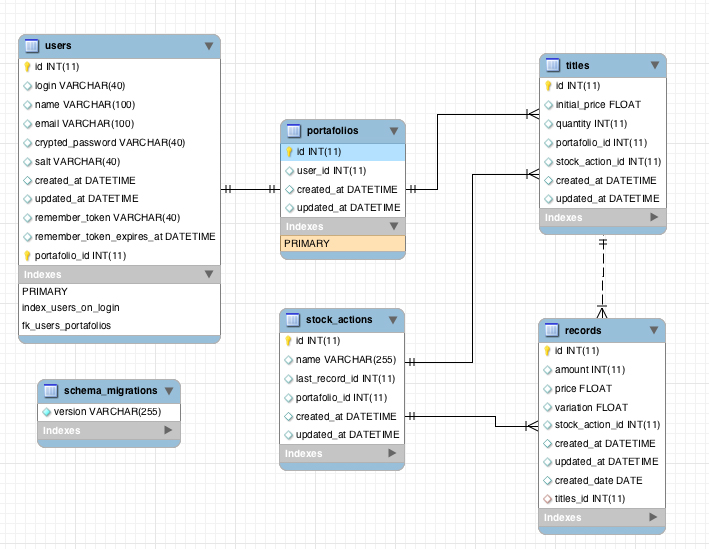
\includegraphics[scale=0.5]{erb_mertd.jpg}
		\caption{Modelo Entidad Relación - Mertd(Mercado 3D)}
	\label{fig:erd}
\end{figure}

Finalmente el modelo \emph{record} es sobre el cual se registran todos los movimientos de las acciones, es decir, sobre el que se hacen las actualizaciones según el estado de una acción, por ejemplo, cada vez que se obtiene información nueva indicando el estado de una acción, un registro nuevo es agregado y guardado en este modelo, luego este registro es usado por otros modelos para calcular el estado de una inversión de forma personalizada.\\

La siguiente porción de código de la aplicación, muestra claramente cómo se puede sacar provecho al utilizar un patrón como \textbf{ActiveRecord}, según este patrón, si existe una tabla \emph{titles} debe haber una clase \emph{Title} asociada, sobre la cual se hace el mapeo.

\begin{verbatim}
	t = Title.new
	t.initial_price = 15250.66
	t.quantity = 10000
	t.portafolio = p #p es un portafolio existente cuya id es 1
	t.stock_action = s_a #s_a es una acción existente cuya id es 15
	t.save
	#otra manera mas corta de hacer este regristro, podría ser:
	#t = Title.new(:initial_price => 15250.66, :quantity => 10000, 
	#			   :portafolio => p, :stock_action => s_a)
	#
\end{verbatim}

A nivel de bases de datos, las anteriores declaraciones son interpretadas de la siguiente manera:

\begin{verbatim}
INSERT INTO titles 
  (initial_price, quantity, portafolio_id, stock_action_id) 
  VALUES (15250.66, 10000, 1, 15);
\end{verbatim}

Cabe resaltar que siempre será más rápido ejecutar directamente el código nativo interpretado por el motor de base de datos, pero en éste caso se opto por la claridad de código y la manipulación de objetos pues no se requirió diseñar consultas que hicieran que la diferencia de tiempos entre uno y otro método fuera considerable.

\subsection{Configuración.}

Al tratarse de una aplicación web, la configuración estuvo enfocada en la determinación de que servidores web utilizar, y que motor de bases de datos, así como la integración de estos con la aplicación.

\subsubsection{Servidor Web - \emph{Clusters}}

En el lado de los servidores, se eligió \textbf{Mongrel}\footnote{Es una libreria HTTP y un servidor web para aplicaciones escritas en \emph{Ruby}. Una característica de \emph{Mongrel} es que usa HTTP plano, en vez de \emph{FastCGI} ó \emph{SCGI}, para comunicarse con otros servidores que podrían estar una capa encima de éste.}, encargado de correr la aplicación web a modo de \emph{clusters},\footnote{Los \emph{Mongrel Clusters} son un conjunto de procesos de \emph{Mongrel} con una configuración común que pueden ser manejados por un servidor \emph{Proxy}} éstos interpretan directamente el código escrito en \emph{Ruby} y responden a peticiones HTPP, cuándo se utiliza este esquema se necesita incluir un \textbf{Proxy Sever}\footnote{Es un servidor que intercepta las conexiones de red que un cliente hace a un servidor de destino para actuar como enrutador.} en la primera capa del servidor web, encargado de enrutar las peticiones HTTP a un determinado \emph{cluster} dependiendo del estado de los mismos, para el desarrollo de la aplicación se eligió \textbf{Nginx}\footnote{http://nginx.net/} como servidor proxy.\\

Los siguientes archivos, representan la configuración actual de la aplicación, tanto para \emph{Mongrel} asi como para \emph{Nginx}\\

Archivo de configuración para los \emph{clusters}, el número de \emph{clusters} esta determinado por el valor de la variable \emph{servers}, el primer \emph{cluster} corre en el puerto especificado en la variable \emph{port}, los puertos de los n-1 restantes \emph{clusters} son determinados incrementando en 1 el valor del puerto del último \emph{cluster} al que se le haya asignado un puerto, en este caso, el primer \emph{cluster} corre en el puerto 8000, y el segundo en el puerto 8001.

\begin{verbatim}
  port: "8000" 
  cwd: /home/mertd/www/mertd/current/
  log_file: log/mongrel.log 
  environment: production 
  address: 127.0.0.1 
  pid_file: log/mongrel.pid 
  servers: 2
  docroot: public 
  user: mertd
  group: mertd 
\end{verbatim}

Archivo de configuración de \emph{Nginx}

\begin{verbatim}
	upstream mertd {
		/* Cada uno de los mongrel clusters, en este caso dos */
		/* Corriendo en los puertos 8000 y 8001 respectivamente */
		server 127.0.0.1:8000; 
		server 127.0.0.1:8001;
	}

	server {
	    listen 80;
	    server_name 127.0.0.1;
	    client_max_body_size 25M;

	    root /home/mertd/www/mertd/current/public/;
	    access_log  /home/mertd/www/mertd/current/log/access.log  main;

	    if (-f $document_root/system/maintenance.html) {
	      rewrite  ^(.*)$  /system/maintenance.html last;
	      break;
	    }

	    location / {
	      proxy_set_header  X-Real-IP  $remote_addr;
	      proxy_set_header  X-Forwarded-For $proxy_add_x_forwarded_for;
	      proxy_set_header Host $http_host;
	      proxy_redirect false;
	      proxy_max_temp_file_size 0;
	      if (-f $request_filename) {
	        break;
	      }
	      if (-f $request_filename/index.html) {
	        rewrite (.*) $1/index.html break;
	      }
	      if (!-f $request_filename) {
	        proxy_pass http://mertd;
	        break;
	      }
	    }

	    error_page   500 502 503 504  /500.html;
	    location = /500.html {
	    root /home/mertd/www/mertd/current/public;
	    }
	 }
\end{verbatim}

\subsubsection{Base de datos}

La integración de la aplicación con la base de datos, es uno de los aspectos en los que \emph{Rails} saca ventaja de su filosofía CoC (\emph{Convention over Configuration}), en este punto sólo es necesario definir que motor de base de datos soportado por \emph{Rails} se utilizará y en 7 líneas de código la integración se define.

\begin{verbatim}
development: 
  adapter: mysql 
  encoding: utf8 
  database: mertd_development 
  username: root 
  password: 
  host: localhost	
\end{verbatim}

\emph{Rails} cuenta con tres tipos de ambientes, las líneas anteriores corresponden a la configuración de la base de datos para el ambiente de \emph{desarrollo} los otros dos son: \emph{producción} (la versión que utilizan los usuarios) y \emph{test}, a partir de ese momento, la base de datos puede ser creada, modificada, o eliminada sin necesidad de utilizar directamente código SQL, la base de datos de \emph{Mertd} fue creada siguiendo un patrón de migraciones\cite{ror:cookbook}\footnote{La base de datos es modificada como si se tratase de una máquina de estados, cada migración agrega, modifica, elimina o actualiza la estructura de la base de datos} para facilitar escabilidad entre base de datos y aplicación.\\

A modo de ejemplo, las siguientes sentencias recrean la creación de la base de datos, y el primer modelo de la aplicación siguiendo el patrón de migraciones.\\

La siguiente tarea crea la base de datos basado en el archivo de configuración.

\begin{verbatim}
  rake db:create 
\end{verbatim}

Como se mencionó anteriormente, la base de datos se modifica basado en migraciones, las siguiente sentencia, muestra como crear y detallar el comportamiento de una migración, en este caso para crear la tabla/modelo usuarios. 

\begin{verbatim}
  script/generate migration create_users
\end{verbatim}

El script anterior genera un archivo en el que se definen las operaciones que se aplicaran a la base de datos cuando la migración sea ejecutada, la siguiente porción de código muestra el contenido de dicho archivo utilizado en \emph{Mertd}

\begin{verbatim}
class CreateUsers < ActiveRecord::Migration
  def self.up
    create_table "users", :force => true do |t|
      t.column :login,                     :string, :limit => 40
      t.column :name,                      :string, :limit => 100
      t.column :email,                     :string, :limit => 100
      t.column :crypted_password,          :string, :limit => 40
      t.column :salt,                      :string, :limit => 40
      t.column :created_at,                :datetime
      t.column :updated_at,                :datetime
      t.column :remember_token,            :string, :limit => 40
      t.column :remember_token_expires_at, :datetime


    end
    add_index :users, :login, :unique => true
  end

  def self.down
    drop_table "users"
  end
end
\end{verbatim}

Para cada migración se debe definir una tarea dependiendo si se realiza la migración o si por el contrario se esta revirtiendo una migración, la migración anterior por ejemplo, para ser revertida utiliza la sentencia \emph{drop\_table}.\\

Finalmente para actualizar la base de datos se corre la migración mediante una tarea \emph{rake}\footnote{Un programa de construcción de \emph{Ruby} con características similares a \emph{make}}.

\begin{verbatim}
  rake db:migrate  #crea la tabla usuarios ("users")
  rake db:rollback #elimina la tabla usuarios ("users")
\end{verbatim}

\subsection{Daemon - \emph{Stock Getter}}

Al ser una aplicación que necesita estar constantemente recolectando datos desde sitios externos, se hizo necesario la implementación de un Demonio ó \textbf{Daemon}\footnote{Léase \textbf{Daemon} en el glosario.} que desarrollara esta tarea, pues una implementación dentro de la aplicación web, al estar corriendo en un mismo proceso, representaría un saturamiento innecesario que podría repercutir en el rendimiento de la aplicación al procesar peticiones HTTP y consecuentemente en la experiencia del usuario.\\

El \emph{Daemon}, se encarga entonces, de recolectar datos nuevos cada 20 minutos mientras que el mercado accionario se encuentre abierto, dicho mercado esta abierto, de Lunes a Vierns de 09:00am a 01:00pm en zona horaria Colombiana (GMT -5), una vez el mercado cierra, el \emph{Daemon} determina la próxima fecha en que el mercado abrirá, calcula los segundos desde el momento actual hasta esa fecha, y entra en estado `dormido' hasta que el mercado vuelva a abrir, y se repita la tarea cada 20 minutos.\\

A continuación se muestra la definición del \emph{Daemon} que recoge los nuevos registros para las acciones en la aplicación. (cabe anotar que se ejectua como un proceso independiente de la aplicación y automatizado.)

\begin{verbatim}
#!/usr/bin/env ruby
require File.expand_path(File.dirname(__FILE__)) + '/../../config/boot' 
rails_root = File.expand_path RAILS_ROOT

ENV["RAILS_ENV"] ||= "production"

Dir.chdir(rails_root) # Change current directory to RAILS_ROOT 
require "config/environment" # Start up rails
require "stock.rb" #loads the stock library.

$running = true
Signal.trap("TERM") do 
  $running = false
end

while($running) do
  #makes work the production logger
  #for debuggin purposes.
  RAILS_DEFAULT_LOGGER.auto_flushing = 1
  s = Stock.new
  col_time = s.time #gets the current colombian time

  if s.open?
    #Hopefully using this statment we dont have to use a monitor.
    ActiveRecord::Base.connection.reconnect!
    s.parsing
    ActiveRecord::Base.logger.info "Getting Stock info at #{col_time}.\n"
    #lets close the logger.
    RAILS_DEFAULT_LOGGER.auto_flushing = 1000
    sleep 1200 #1200 secs = 20 mins.
  else
    if(col_time > s.close_time)
      Record.delete_last_history_day(s)
      ActiveRecord::Base.logger.info( 
	          "Deleting last day records, last day => #{s.last_day}")
    end
    ActiveRecord::Base.logger.info "Sleeping at #{col_time}.\n"
    RAILS_DEFAULT_LOGGER.auto_flushing = 1000
    sleep s.secs_til_open #sleeps til next open day.
  end

end
\end{verbatim}

Al ser un proyecto con fines académicos el \emph{Daemon} no reconoce días festivos.

\subsection{\emph{TDD Cycle}}

Siguiendo una metodología como \textbf{TDD}(\emph{Test Driven Development} ó Desarrollo Guiado por Pruebas) se realizó el desarrollo del núcleo de la aplicación, esta práctica de programación se usa generalmente para lograr un código limpio y funcional, la idea es que se utilicen las especificaciones/requerimientos definidos anteriormente, para que sean traducidos en pruebas, cada vez que el conjunto de pruebas que definen un requerimiento pasan, se garantiza que la especificación ha sido implementada correctamente. Otro punto importante, es el de hacer pruebas pequeñas con el fin de determinar bajo que condiciones se introduce un error, ó cuando falla la aplicación.\\

El ciclo entonces consiste en que para cada especificación, se debe:
\begin{enumerate}
\item Escribir el test antes de la implementación.
\item Escribir la implementación.
\item Correr el conjunto de tests.
\item Corregir errores en caso de que la prueba falle, de otro modo, avanzar a la siguiente especificación.
\end{enumerate}

A continuación, se muestra el código para el test e implementación, de la especificación para la creación/actualización de títulos con datos válidos.\\

\begin{verbatim}
#Titles controller specification. Test File.

...

describe "responding to POST create" do

   def do_post
      post :create, :title => @params[:title], 
                    :portafolio_id => @params[:portafolio_id], 
                    :name => @params[:name]
   end

   before do
     Portafolio.stub!(:find).and_return(@mock_portafolio)
     @mock_stock = mock_model(StockAction, :save => true, 
                              :name => "ALMACENES EXITO", :id => 1)
     @params = {:title => {:quantity => 301, :initial_price => 14000.23}, 
                :name => "Exito", :portafolio_id => 1}
     StockAction.stub!(:find_with_short_name).with
                      (@params[:name]).and_return(@mock_stock)
   end

   describe "receiving existing title and valid params" do
     it "should update the title" do
       @mock_title = mock_model(Title, :save => true, 
                                :portafolio_id => 1, :stock_action_id => 1)
       Title.should_receive(:find).and_return(@mock_title)
       @mock_title.should_receive(:update_attr_average).with
                   (@params[:title][:quantity], 
                   @params[:title][:initial_price]).and_return(true))
       do_post
       response.should redirect_to(portafolio_path(@mock_portafolio))
     end
   end
end

...
\end{verbatim}

Con el conjunto de tests definidos, se procede a escribir la implementación para una determinada especificación, en este caso, para la creación/actualización de títulos dentro de un portafolio; A continuación se muestra el código perteneciente a dicha especificación, según el test.

\begin{verbatim}
def create
  stock_action = StockAction.find_by_short_name(params[:name]) 
  respond_to do |format|
    if stock_action
      t = Title.find(:first, 
          :conditions => ["portafolio_id = ? and stock_action_id = ?", 
                          @portafolio.id, stock_action.id])
      if t
        quantity = params[:title][:quantity]
        price = params[:title][:initial_price]
        if t.update_attr_average(quantity.to_i, price.to_f)
          format.html { redirect_to(portafolio_path(@portafolio)) }
        else
          format.html { redirect_to :back }
          flash[:error] = 'Los datos ingresados no son válidos.'
        end
      else
        @title = @portafolio.titles.build(params[:title])    
        @title.stock_action = stock_action
        if @title.save
          format.html { redirect_to(portafolio_path(@portafolio)) }
        else
          format.html { redirect_to :back }
          flash[:error] = 'Los datos ingresados no son válidos'
        end
      end
    else
      format.html { redirect_to :back }
      flash[:error] = 'La acción no existe.'
    end
  end
end
\end{verbatim}

De esta manera, se itera a través de todas las especificaciones, para consecuentemente escribir, tests e implementación, asegurando que la aplicación hace lo que debe hacer.


\section{Desarrollo Contenidos 3D}
La arquitectura dentro de una escena en \textbf{Unity3D} consiste en un conjunto de \textbf{GameObjects} que interactúan entre si para mostrar un evento/animación en una escena; Dichos objetos se comunican, basándose en una jerarquía de objetos, donde la traslación/rotación/escalamiento de un padre afecta directamente a los hijos Figura\ref{fig:jerarq}.\\


\begin{figure}[h]
	\centering
		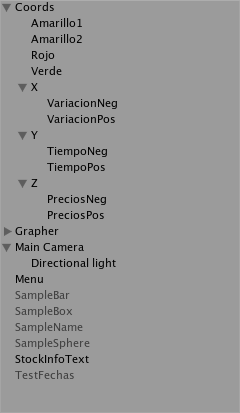
\includegraphics[scale=0.5]{parenting.png}
		\caption{Jerarquía de Objetos en Unity3D.}
	\label{fig:jerarq}
\end{figure}

En este caso, si se rotara/escalára/moviera el objeto `Coords', a su vez a los objetos que se encuentran dentro de `Coords' también se les aplicaría la transformación.\\

Se decidió entonces dividir el programa en 3 grandes módulos principales para facilitar tanto desarrollo como mantenimiento de los contenidos 3D, Dichos modulos le envian información a los otros para renderizar los contenidos 3D. Figura\ref{fig:modules}\\

\begin{figure}[h]
	\centering
		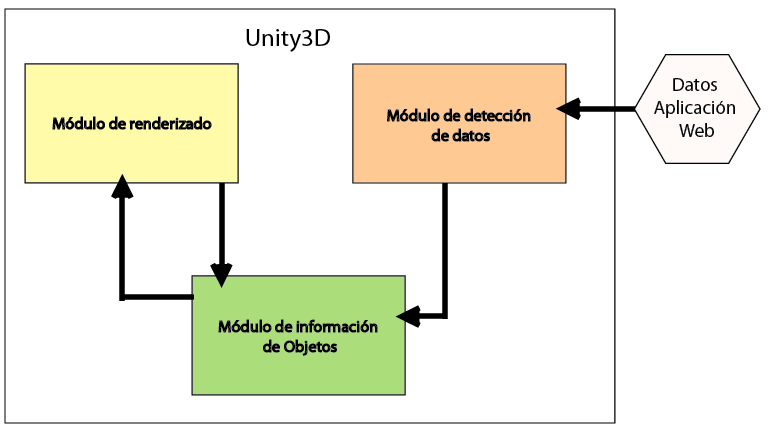
\includegraphics[scale=0.5]{ArquitecturaUnity.png}
		\caption{Arquitectura de los contenidos 3D}
	\label{fig:modules}
\end{figure}


\subsection{Módulo de detección de datos e información del exterior:}
Este módulo se encarga de recibir la información que tiene cada acción que proviene desde la aplicación Web parseándola y organizándola para que los otros módulos de la aplicación la entiendan; posteriormente carga en memoria dicha información para así utilizarla apropiadamente en el tipo de gráfico que se esta renderizando.\\

Este módulo solo es usado cada vez que se le inyectan datos a los contenidos 3D ó cada vez que el usuario pide cambiar el tipo de gráfica a mostrar.\\

\subsection{Modulo de información de Objetos:}
Este módulo se encarga de recolectar la información almacenada en memoria y cargar para cada objeto que se va a mostrar en la escena, la información pertinente del mismo.\\

Este módulo se encarga del manejo de menús y todo lo que tiene que ver con la interacción del usuario con la aplicación, es llamado constantemente cada vez que el usuario desea averiguar información relevante de una acción, y  se comunica una sola vez con el módulo de detección de datos e información del exterior.\\

\subsection{Módulo de renderizado de escena (\emph{Grapher}):}

Finalmente, éste módulo se encarga de lo que es el dibujado de la información proveniente del modulo de información de objetos; éste módulo nunca se entiende con el módulo de datos e información del exterior.\\
 
Para graficar la escena, se recorren todos los nodos que posee el módulo de información y se gráfica (dependiendo del tipo de gráfico) cada nodo.\\


Cabe aclarar que se debe hacer un `vaciado de hijos' del objeto \emph{Grapher} cada vez que se visualizan contenidos, para no introducir \textbf{leaks}\footnote{Ocurre cuando un bloque de memoria reservada no es liberada en un programa de computación. Comúnmente ocurre porque se pierden todas las referencias a esa área de memoria antes de haberse liberado. Dependiendo de la cantidad de memoria perdida y el tiempo que el programa siga en ejecución, este problema puede llevar al agotamiento de la memoria disponible en la máquina.} de memoria.\\



Basicamente 4 tipos de gráficos fueron los que se decidieron desarrollar: Barras, Espiral, Superficie y el Campo. Cada gráfica ofrece información relevante para cada tipo de variable que se esta analizando. \\

\textbf{Barras} [\ref{fig:Barras}:] Son las típicas barras que se pueden encontrar en cualquier visualización de acciones, pero con el valor agregado de que permiten ver el comportamiento de una o varias acciones a través del tiempo.\\

Estas barras muestran variables como el porcentaje de variación, Cantidad negociada, y Precio; Dichos valores son trabajados de modo percentil para poder comparar las otras acciones que tienen precios diferentes, pues una acción puede valer \$5 mientras que otra puede valer \$20000.\\


\begin{figure}[h]
	\centering
		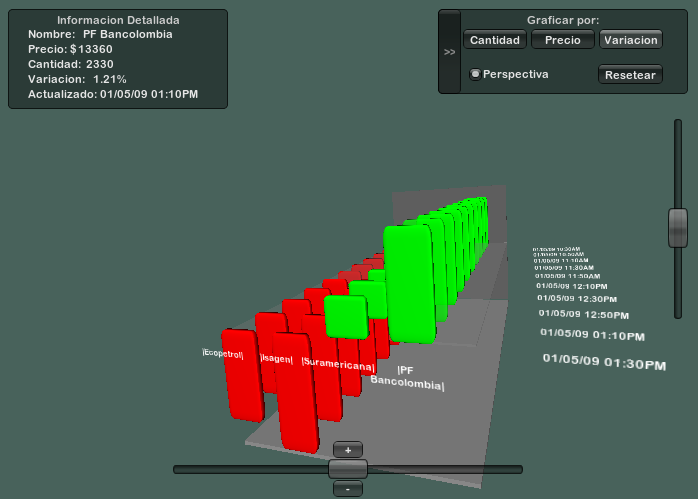
\includegraphics[scale=0.5]{Barras.png}
		\caption{Ejemplo de Visualización por Barras.}
	\label{fig:Barras}
\end{figure}


\textbf{Espiral} [\ref{fig:Espiral}]: Este tipo de gráfica permite comparar rendimientos de varias acciones por medio del porcentaje de variación de cada una en un momento determinado, es el único tipo de gráfico que no permite comparar acciones a través del tiempo, pues lo único que interesa en este gráfico, es determinar de una manera fácil y rápida que acciones están generando mas rentabilidad, cuales están perdiendo y cuales están invariantes en un tiempo dado.\\

\begin{figure}[h]
	\centering
		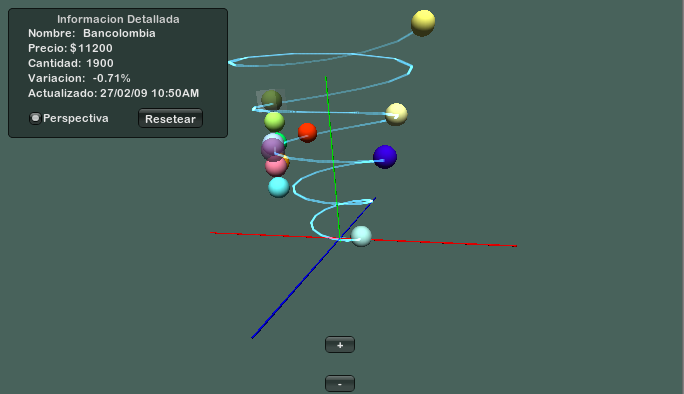
\includegraphics[scale=0.5]{Espiral.png}
		\caption{Ejemplo de Visualización por Espiral.}
	\label{fig:Espiral}
\end{figure}


\textbf{Superficie} [\ref{fig:Superficie}]: Este tipo de gráfico también compara rentabilidades de dos o mas acciones a través del tiempo, con respecto a la mayor/menor rentabilidad de todas las acciones en un momento determinado  mientras que genera una superficie 3D que describe el comportamiento de la bolsa a medida que transcurre el tiempo.\\

\begin{figure}[h]
	\centering
		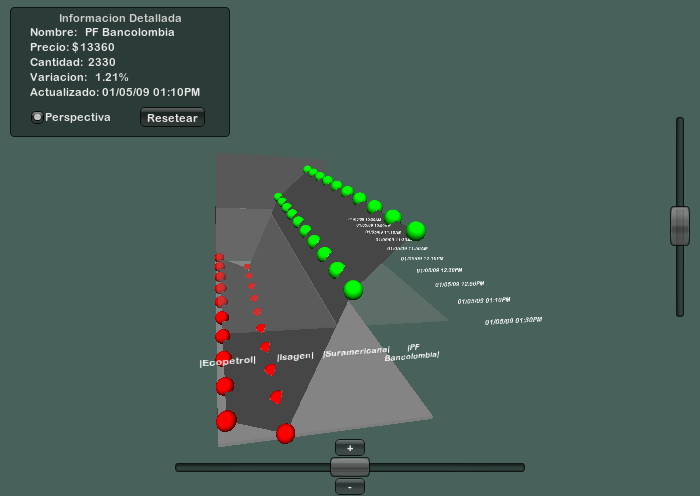
\includegraphics[scale=0.5]{Superficie.png}
		\caption{Ejemplo de Visualización por superficies de rentabilidad.}
	\label{fig:Superficie}
\end{figure}

\textbf{Campo} [\ref{fig:Campo}]: Es el tipo de gráfico mas complejo que se realizó, pues en este gráfico se comparan variables de Cantidad Vs Rentabilidad a través del tiempo, entonces por medio de estas variables se puede inferir si una acción se esta tranzando en la bolsa en mucha cantidad o no y si dicha acción esta siendo rentable; Este gráfico provee una serie de `zonas' que ayudan al usuario a entender el estado de las acciones en un momento dado, y así inferir facilmente si la acción esta generando pérdidas o ganancias y si esta muy o poco demandada\\

\begin{figure}[h]
	\centering
		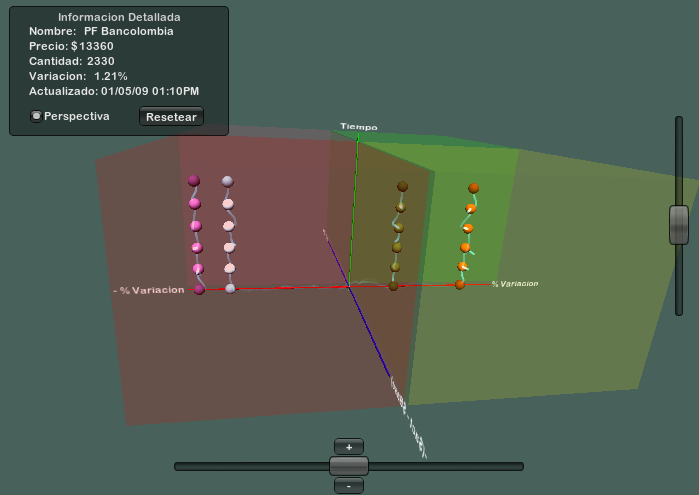
\includegraphics[scale=0.5]{Campo.png}
		\caption{Ejemplo de Visualización por Campos.}
	\label{fig:Campo}
\end{figure}
 

\section{Desarrollo protocolo de comunicación.}

Para el conectar los contenidos 3D con toda la aplicación web, como se mencionó en secciones anteriores, se desarrolló un protocolo escrito en \emph{Javascript}, puesto que \emph{Unity3D} permite el llamado a funciones implementadas dentro del motor por medio de este lenguaje.\\ 

Fue así como por medio de paso de mensajes y llamadas a funciones, se implementó el protocolo de comunicaciones, dicho protocolo actúa como canal sobre el que pasan mensajes a través de funciones nativas de \emph{Javascript} desde la aplicación web (\emph{Ruby} cuenta con una librería especifica para serializar objetos a \emph{Javascript}) a un Objeto \emph{Unity3D} que arroja el \emph{player}, dichas funciónes permiten hacer llamadas nativas a funciones de los contenidos 3D, facilitando este proceso que en un principio pareciera ser más tedioso.\\

El principal problema que se presentó a la hora de diseñar el protocolo fue que el contenido  \emph{HTML} se cargaba antes y mas rápido que el contenido en 3D, lo que conducia eventualmente a la perdida de mensajes y a la incorrecta graficación de los datos. Para solucionar este problema se implementó una llamada desde el contenido 3D a la aplicación web  a través del protocolo que indica cuando un contenido esta listo para recibir datos, y de esta manera graficar correctamente los datos.

A continuación se muestra la parte del protocolo y la función implementada desde el motor, que indica cuando el contenido esta listo para recibir y enviar mensajes.

\begin{verbatim}
write: function (elementId) {
    if(this.detectUnityWebPlayer()) {
        document.write(this.writeEmbedDOM());
        this.findEar();
        return true;
    } else {
        if(this.getAttribute('altHTML') != "") {
            document.write(this.getAttribute('altHTML'));
        } else if(this.getAttribute('redirectUrl') != "") {
            document.location.replace(this.getAttribute('redirectUrl'));
        }
    }
    return false;
},

findEar: function () {
    this.unityEar = "";
    if (navigator.appVersion.indexOf("MSIE") != -1 && 
        navigator.appVersion.toLowerCase().indexOf("win") != -1) {
        this.unityEar = document.getElementById(this.getAttribute('id')+"_object");
    } else if (navigator.appVersion.toLowerCase().indexOf("safari") != -1) {
        this.unityEar = document.getElementById(this.getAttribute('id')+"_object")
    } else {
        this.unityEar = document.getElementById(this.getAttribute('id')+"_embed");
    }
    document.Unity = this.unityEar;
},
   
msg: function (unObj, unFunc, unVar) {
    this.unityEar.SendMessage(unObj, unFunc, unVar);
}
\end{verbatim}

La siguiente porción de código manda una señal hacia el protocolo implementado en \emph{Javascript}, indicando que la aplicación esta lista para renderizar contenidos.\\

\begin{verbatim}
//Funcion implementada en Unity3D
function Update() {
    if(Application.GetStreamProgressForLevel(0) == 1 && !finishedLoadingApp){
        Application.ExternalCall("FinishedLoadingApp");
        finishedLoadingApp = true;
    }
}
\end{verbatim}
\section{\emph{Deployment}}



\section{SCM}